\newpage
\subsection{Geração da Trajetória}

A trajetória do manipulador foi definida diretamente no espaço cartesiano a partir das dimensões da bandeira e da posição de seu centro.

O centro da bandeira foi definido como

\[
P_c=
\begin{bmatrix}
X_c\\
Y_c\\
Z_c
\end{bmatrix}
=
\begin{bmatrix}
0,65\\
0,00\\
0,45
\end{bmatrix}
m.
\]

\subsubsection{Interpolação da Trajetória}

A trajetória da bandeira foi inicialmente definida por um conjunto discreto de
pontos cartesianos correspondentes aos vértices do retângulo, do losango e aos
pontos amostrados da circunferência e do arco. Entretanto, o manipulador não pode
se deslocar instantaneamente entre duas posições consecutivas, pois isso
implicaria velocidades infinitas e movimentos fisicamente inviáveis.

Assim, foi utilizada uma técnica de interpolação para gerar posições
intermediárias entre os pontos definidos. A interpolação transforma um conjunto
discreto de coordenadas em uma trajetória contínua, permitindo que o efetuador
descreva um movimento suave ao longo do tempo.

Neste projeto, a interpolação foi realizada diretamente no espaço cartesiano.
Essa escolha foi motivada pela necessidade de preservar a geometria da tarefa de
pintura. Como o objetivo consiste em reproduzir os contornos da bandeira, a
interpolação cartesiana assegura que os lados do retângulo e do losango sejam
percorridos como segmentos de reta, enquanto o círculo mantém sua forma
geométrica original.

Após a geração dos pontos interpolados, cada posição cartesiana foi convertida
para o espaço articular por meio da cinemática inversa do manipulador TX90,
assim, obtendo as configurações necessárias para a execução da tarefa.

\subsubsection{Retângulo Externo}

O retângulo possui largura $w_R = 0,70\,m$ e altura $h_R = 0,5\,m$.
\par O primeiro vértice é calculado por
\[
p_1=
\begin{bmatrix}
X_c\\
Y_c-\frac{w_R}{2}\\
Z_c+\frac{h_R}{2}
\end{bmatrix}.
\]

Substituindo os valores:
\[
p_1=
\begin{bmatrix}
0,65\\
0-\frac{0,70}{2}\\
0,45+\frac{0,5}{2}
\end{bmatrix}
=
\begin{bmatrix}
0,65\\
-0,35\\
0,70
\end{bmatrix}
m.
\]

O segundo vértice é
\[
p_2=
\begin{bmatrix}
0,65\\
0,35\\
0,70
\end{bmatrix}
m.
\]

O terceiro vértice é
\[
p_3=
\begin{bmatrix}
0,65\\
0,35\\
0,20
\end{bmatrix}
m.
\]

O quarto vértice é
\[
p_4=
\begin{bmatrix}
0,65\\
-0,35\\
0,20
\end{bmatrix}
m.
\]

Assim, a trajetória do retângulo é definida pela sequência
\[
P_R=
\{p_1,p_2,p_3,p_4,p_1\}.
\]

\subsubsection{Losango}

O losango possui largura $w_L = 0,58\,m$ e altura $h_L=0,38\,m$.
O vértice superior é
\[
p_5=
\begin{bmatrix}
0,65\\
0\\
0,45+\frac{0,38}{2}
\end{bmatrix}
=
\begin{bmatrix}
0,65\\
0\\
0,64
\end{bmatrix}
m.
\]

O vértice direito é
\[
p_6=
\begin{bmatrix}
0,65\\
0+\frac{0,58}{2}\\
0,45
\end{bmatrix}
=
\begin{bmatrix}
0,65\\
0,29\\
0,45
\end{bmatrix}
m.
\]

O vértice inferior é
\[
p_7=
\begin{bmatrix}
0,65\\
0\\
0,45-\frac{0,38}{2}
\end{bmatrix}
=
\begin{bmatrix}
0,65\\
0\\
0,26
\end{bmatrix}
m.
\]

O vértice esquerdo é
\[
p_8=
\begin{bmatrix}
0,65\\
-0,29\\
0,45
\end{bmatrix}
m.
\]

A trajetória do losango é definida por
\[
P_L=
\{p_5,p_6,p_7,p_8,p_5\}.
\]

\subsubsection{Círculo Central}

O círculo possui raio $r_C=0,123\,m$.
\par Sua trajetória foi parametrizada por

\[
P_C(\theta)=
\begin{bmatrix}
0,65\\
0+0,123\cos(\theta)\\
0,45+0,123\sin(\theta)
\end{bmatrix},
\]

com

\[
\theta
\in
\left[
\frac{\pi}{2},
-\frac{3\pi}{2}
\right].
\]

O primeiro ponto do círculo é obtido para

\[
\theta=\frac{\pi}{2}
\]

resultando em

\[
P_C
=
\begin{bmatrix}
0,65\\
0\\
0,57
\end{bmatrix}
m.
\]

\subsubsection{Arco}

O arco no centro do círculo possui raio $r_A=0,289\,m$.
Sua trajetória foi parametrizada por

\[
P_A(\theta)=
\begin{bmatrix}
0,65\\
-0,07+0,289\cos(\theta)\\
0,20+0,289\sin(\theta)
\end{bmatrix},
\]

com

\[
\theta
\in
\left[
1.7359,
0.8597
\right]rad.
\]

\subsubsection{Interpolação Cartesiana}

Entre dois pontos consecutivos da trajetória foi utilizada interpolação linear para definir a geometria, combinada com uma lei temporal LSPB para definir como o ponto avança ao longo do segmento.
Considerando um ponto inicial \(P_i\) e um ponto final \(P_f\), a posição instantânea é dada por
\[
P(t)
=
P_i
+
\lambda(t)
\left(
P_f-P_i
\right),
\]

onde
\[
0 \le \lambda(t) \le 1.
\]

Como exemplo, para o primeiro lado do retângulo,
\[
P_i=p_1=
\begin{bmatrix}
0,65\\
-0,35\\
0,70
\end{bmatrix}
\]

e
\[
P_f=p_2=
\begin{bmatrix}
0,65\\
0,35\\
0,70
\end{bmatrix}.
\]

Logo,

\[
P_f-P_i=
\begin{bmatrix}
0\\
0,70\\
0
\end{bmatrix}.
\]

A trajetória desse segmento é

\[
P(t)
=
\begin{bmatrix}
0,65\\
-0,35\\
0,70
\end{bmatrix}
+
\lambda(t)
\begin{bmatrix}
0\\
0,70\\
0
\end{bmatrix}.
\]

Portanto,

\[
P(t)
=
\begin{bmatrix}
0,65\\
-0,35+0,70\lambda(t)\\
0,70
\end{bmatrix}.
\]

Esse procedimento foi repetido para todos os segmentos do retângulo, do losango e para os pontos discretizados do círculo.

\begin{table}[H]
\centering
\caption{Pontos cartesianos utilizados para a geração da trajetória da bandeira.}
\label{tab:pontos_bandeira}
\begin{tabular}{c|c|c|c|c}
\hline
Índice &
Retângulo $(x,y,z)$ [m] &
Losango $(x,y,z)$ [m] &
Círculo $(x,y,z)$ [m] &
Arco $(x,y,z)$ [m]\\
\hline

1 &
$(0.65,-0.35,0.70)$ &
$(0.65,0.00,0.64)$ &
$(0.65,0.000,0.573)$ &
$(0.65,-0.117,0.485)$ \\

2 &
$(0.65,0.35,0.70)$ &
$(0.65,0.29,0.45)$ &
$(0.65,0.020,0.571)$ &
$(0.65,-0.111,0.486)$ \\

3 &
$(0.65,0.35,0.20)$ &
$(0.65,0.00,0.26)$ &
$(0.65,0.039,0.566)$ &
$(0.65,-0.105,0.487)$ \\

4 &
$(0.65,-0.35,0.20)$ &
$(0.65,-0.29,0.45)$ &
$(0.65,0.057,0.559)$ &
$(0.65,-0.098,0.487)$ \\

5 &
$(0.65,-0.35,0.70)$ &
$(0.65,0.00,0.64)$ &
$(0.65,0.074,0.548)$ &
$(0.65,-0.092,0.488)$ \\

\hline
\end{tabular}
\end{table}

\subsubsection{Trajetória Circular}

O círculo central da bandeira foi definido diretamente por sua parametrização angular.
\par O raio utilizado foi
\[
r_C = 0.1225\;m.
\]

A trajetória foi parametrizada por
\[
P_C(\theta)=
\begin{bmatrix}
x(\theta)\\
y(\theta)\\
z(\theta)
\end{bmatrix}
=
\begin{bmatrix}
0.65\\
0.1225\cos(\theta)\\
0.45+0.1225\sin(\theta)
\end{bmatrix},
\]

sendo
\[
\theta \in
\left[
\frac{\pi}{2},
-\frac{3\pi}{2}
\right].
\]

Dessa forma, o efetuador percorre uma circunferência completa no plano \(YZ\), mantendo a coordenada \(X\) constante.

\begin{table}[H]
\centering
\caption{Pontos característicos da trajetória circular.}
\label{tab:circulo}
\begin{tabular}{c c c c c}
\hline
Ponto & $\theta$ (rad) & $x$ (m) & $y$ (m) & $z$ (m) \\
\hline

$P_1$ &
$\frac{\pi}{2}$ &
0.65 &
0.000 &
0.573 \\

$P_2$ &
0 &
0.65 &
0.123 &
0.450 \\

$P_3$ &
$-\frac{\pi}{2}$ &
0.65 &
0.000 &
0.327 \\

$P_4$ &
$-\pi$ &
0.65 &
-0.123 &
0.450 \\

$P_5$ &
$-\frac{3\pi}{2}$ &
0.65 &
0.000 &
0.573 \\

\hline
\end{tabular}
\end{table}

O resultado esperado coincide com a figura a seguir, que contém os vértices e a trajetória definida.

\begin{figure}[H]
    \centering
    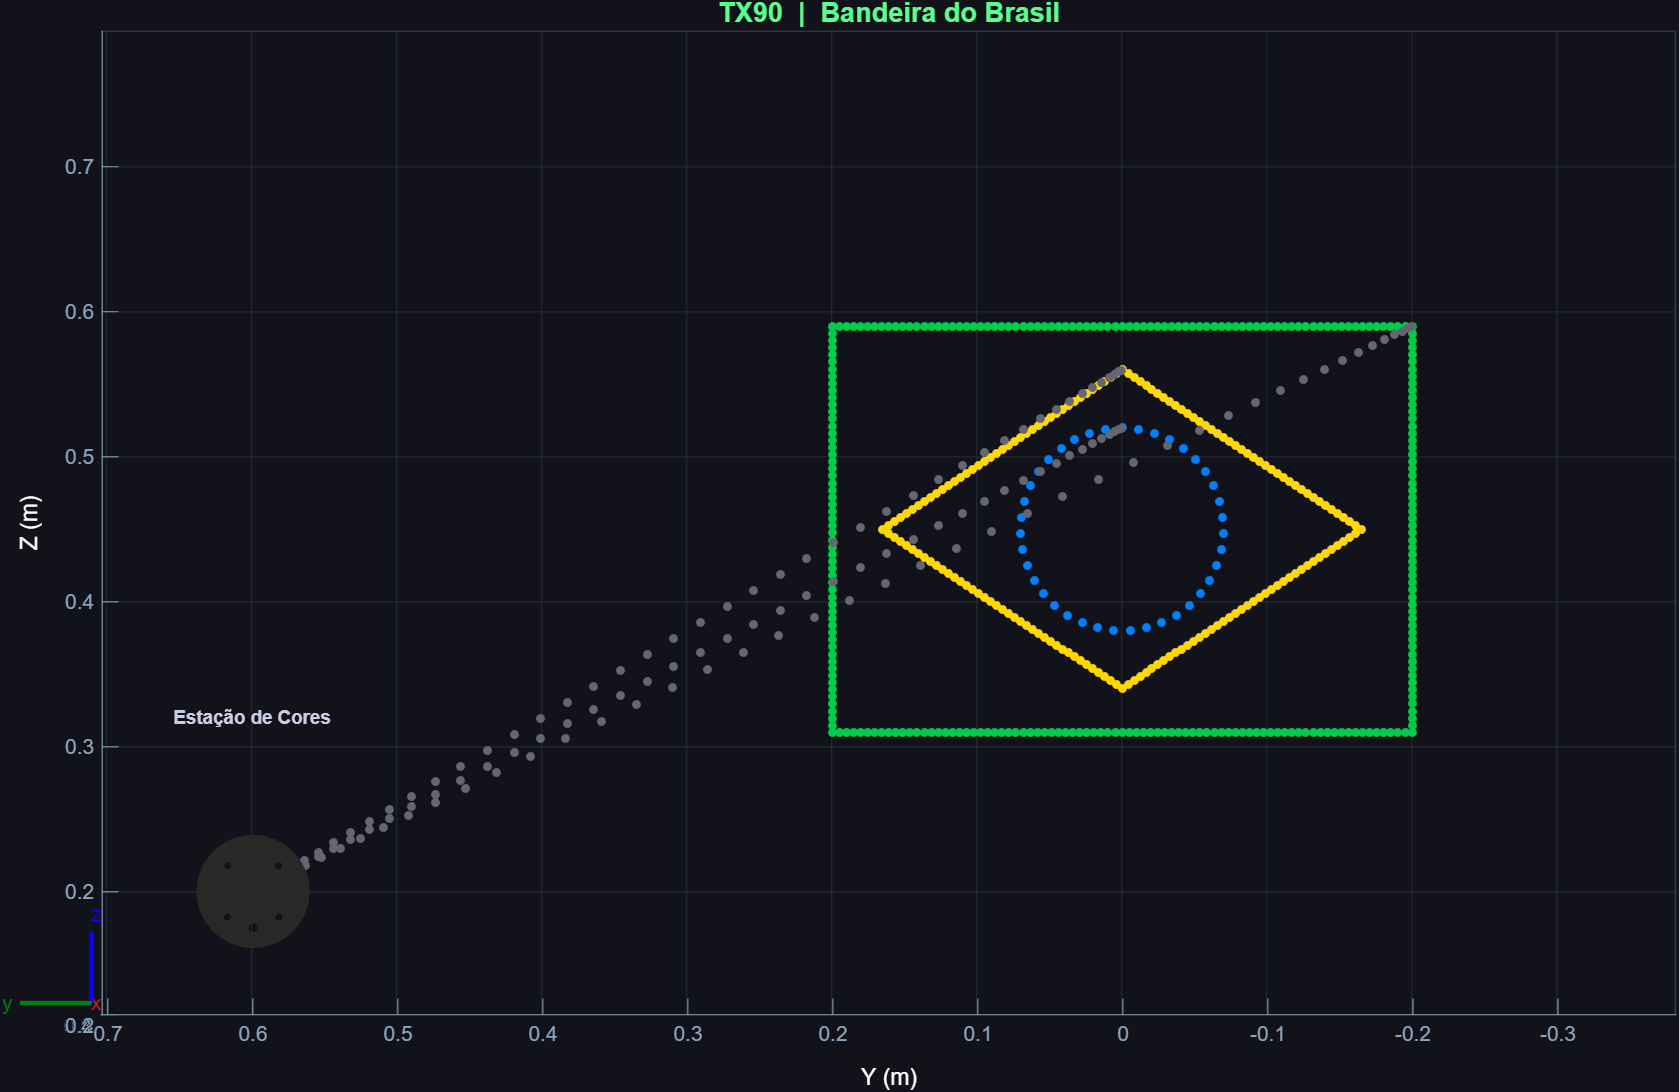
\includegraphics[width=0.8\linewidth]{Imagens/Bandeira_sim-2.png}
    \caption{Trajetória dos pontos da bandeira do Brasil}
\end{figure}

\subsubsection{Conversão da trajetória para o espaço articular}

Considerando dois pontos consecutivos da trajetória, \(P_i\) e \(P_f\), a posição
intermediária é obtida por
\[
P(t)=P_i+\lambda(t)\left(P_f-P_i\right),
\]
em que
\[
0 \leq \lambda(t) \leq 1.
\]

O parâmetro $\lambda(t)$ foi obtido a partir de uma coordenada de caminho $s(t)$. Para um segmento de comprimento $L$, com tempo total $T$, tempo de aceleração $t_b$, velocidade de cruzeiro $v$ e aceleração $a$, foi utilizado o perfil LSPB apresentado na disciplina \cite{alkmin2026trajetoria}:
\begin{equation}
s(t)=
\begin{cases}
\dfrac{1}{2}at^2, & 0\leq t\leq t_b,\\[4pt]
\dfrac{1}{2}at_b^2+v(t-t_b), & t_b<t<T-t_b,\\[4pt]
L-\dfrac{1}{2}a(T-t)^2, & T-t_b\leq t\leq T.
\end{cases}
\label{eq:lspb_posicao}
\end{equation}

As relações usadas para fechar o perfil são
\begin{equation}
v=a t_b,
\qquad
L=v(T-t_b).
\label{eq:lspb_relacoes}
\end{equation}

Para compatibilizar o perfil contínuo com o período de amostragem \(\Delta t=0{,}04\,\mathrm{s}\), o tempo total e o tempo de aceleração são definidos por

Para representar o perfil em intervalos de \(\Delta t=0{,}04\,\mathrm{s}\), foram considerados

\[
T=n\Delta t
\qquad \text{e} \qquad
t_b=n_b\Delta t,
\]

em que \(n\) e \(n_b\) são números inteiros. A partir das relações do perfil LSPB, a velocidade e a aceleração de cada segmento são calculadas por

\[
v=\frac{L}{T-t_b},
\qquad
a=\frac{v}{t_b}.
\]

Os valores de \(T\) e \(t_b\) são escolhidos de forma que

\[
v\leq v_{\max}
\qquad \text{e} \qquad
a\leq a_{\max}.
\]

Durante a ação pintura foram utilizados \(v_{\max}=0{,}12\,\mathrm{m/s}\) e \(a_{\max}=0{,}30\,\mathrm{m/s^2}\). Para os deslocamentos entre a estação e a bandeira, foram adotados \(v_{\max}=0{,}35\,\mathrm{m/s}\) e \(a_{\max}=0{,}60\,\mathrm{m/s^2}\).

Pelas equações do perfil, verifica-se que \(s(0)=0\), \(s(T)=L\) e que a velocidade é nula no início e no final do movimento. Dessa forma, a posição, e a velocidade permanecem contínuas, enquanto a velocidade e a aceleração respeitam os limites já definidos.

Para converter a trajetória cartesiana para o espaço articular, determina-se, em cada instante, um vetor de juntas \(q(t)\) que obedeça a:

\[
{}^{0}T_{TCP}\bigl(q(t)\bigr)={}^0T_d(t),
\]

no qual \({}^0T_d(t)\) representa a pose desejada do TCP. Entre as possíveis soluções da cinemática inversa, é utilizada a configuração mais próxima da anterior, evitando mudanças muito bruscas entre configurações do manipulador.

A solução pode ser verificada reconstruindo a pose pela cinemática direta. Para isso, são calculados o erro de posição,

\[
e_p(t)=
\left\|
p_d(t)-p_{FK}\bigl(q(t)\bigr)
\right\|
\]

e o erro de orientação,

\[
e_R(t)=
\cos^{-1}
\left(
\frac{
\operatorname{tr}\!\left[R_d^T(t)R_{FK}\bigl(q(t)\bigr)\right]-1
}{2}
\right).
\]

\subsubsection{Preenchimento das formas em serpentina}

Além do traçado dos contornos, foi implementada a opção de \emph{preenchimento}
das regiões coloridas da bandeira, ativada pelo parâmetro
\texttt{PREENCHER\_BANDEIRA}. O preenchimento reproduz a forma como uma pistola de
pintura cobre uma superfície: por meio de passadas paralelas que varrem toda a
área, técnica conhecida como varredura em serpentina (ou \textit{boustrophedon}).

A região de cada forma é decomposta em uma sequência de faixas horizontais,
espaçadas verticalmente por um passo $\Delta z$ (parâmetro \texttt{PASSO\_LEQUE}).
Em cada faixa, o efetuador percorre a largura da forma de uma borda à outra,
alternando o sentido a cada nível --- da esquerda para a direita em uma faixa e da
direita para a esquerda na seguinte ---, de modo a cobrir toda a superfície sem
deslocamentos desperdiçados. A meia-largura da forma em cada altura $z$, medida a
partir do centro, é dada por uma função $\ell(z)$ específica de cada geometria:

\[
\ell_{\text{ret}}(z)=\frac{w_R}{2},
\qquad
\ell_{\text{los}}(z)=\frac{w_L}{2}\left(1-\frac{|z|}{h_L/2}\right),
\qquad
\ell_{\text{cir}}(z)=\sqrt{R_C^{\,2}-z^2},
\]

isto é, largura constante para o retângulo, decaimento linear para o losango e a
semicorda para o círculo. Cada passada é então percorrida com o mesmo perfil
temporal LSPB descrito anteriormente, o que faz a velocidade se anular nas viradas
e concentra picos de torque nesses instantes.

A faixa branca, por ser curva, não é preenchida por passadas retas, mas por
\emph{arcos concêntricos}: o raio varia entre $R_{\text{arco}}\pm L_{\text{faixa}}/2$
em passos de $\Delta z$, alternando-se o sentido angular a cada arco e ligando arcos
vizinhos por um curto trecho radial. Como todas as formas estão no mesmo plano $X$,
aplica-se ainda um pequeno deslocamento em profundidade a cada camada de cor
(parâmetro \texttt{ESPESSURA\_CAMADA}), representando a espessura da tinta e evitando
que cores sobrepostas conflitem na renderização.

O preenchimento aumenta consideravelmente o número de pontos da trajetória --- de
cerca de $1\,700$ no modo de contorno para vários milhares ---, porém não altera
nenhuma etapa posterior: a cinemática inversa, a dinâmica e o controle consomem a
mesma estrutura de trajetória, apenas com mais pontos a processar.

A Figura~\ref{fig:preenchimento} mostra o resultado do preenchimento executado pelo
manipulador: em (a) veem-se as passadas paralelas em serpentina cobrindo cada
região, e em (b) a bandeira já concluída, com o losango, o círculo e a faixa branca
preenchidos sobre o fundo verde.

Vale ressaltar que os calculos em serpentina foram feitos como uma forma extra ao objetivo 
principal do projeto, e feitos apenas para fins de demonstração e estudo de diferentes trajetórias.
Portanto, na continuação do relatório, os resultados apresentados serão apenas para a trajetória de contorno da bandeira.

\begin{figure}[H]
    \centering
    \subfloat[Passadas em serpentina cobrindo as regiões da bandeira.]{%
        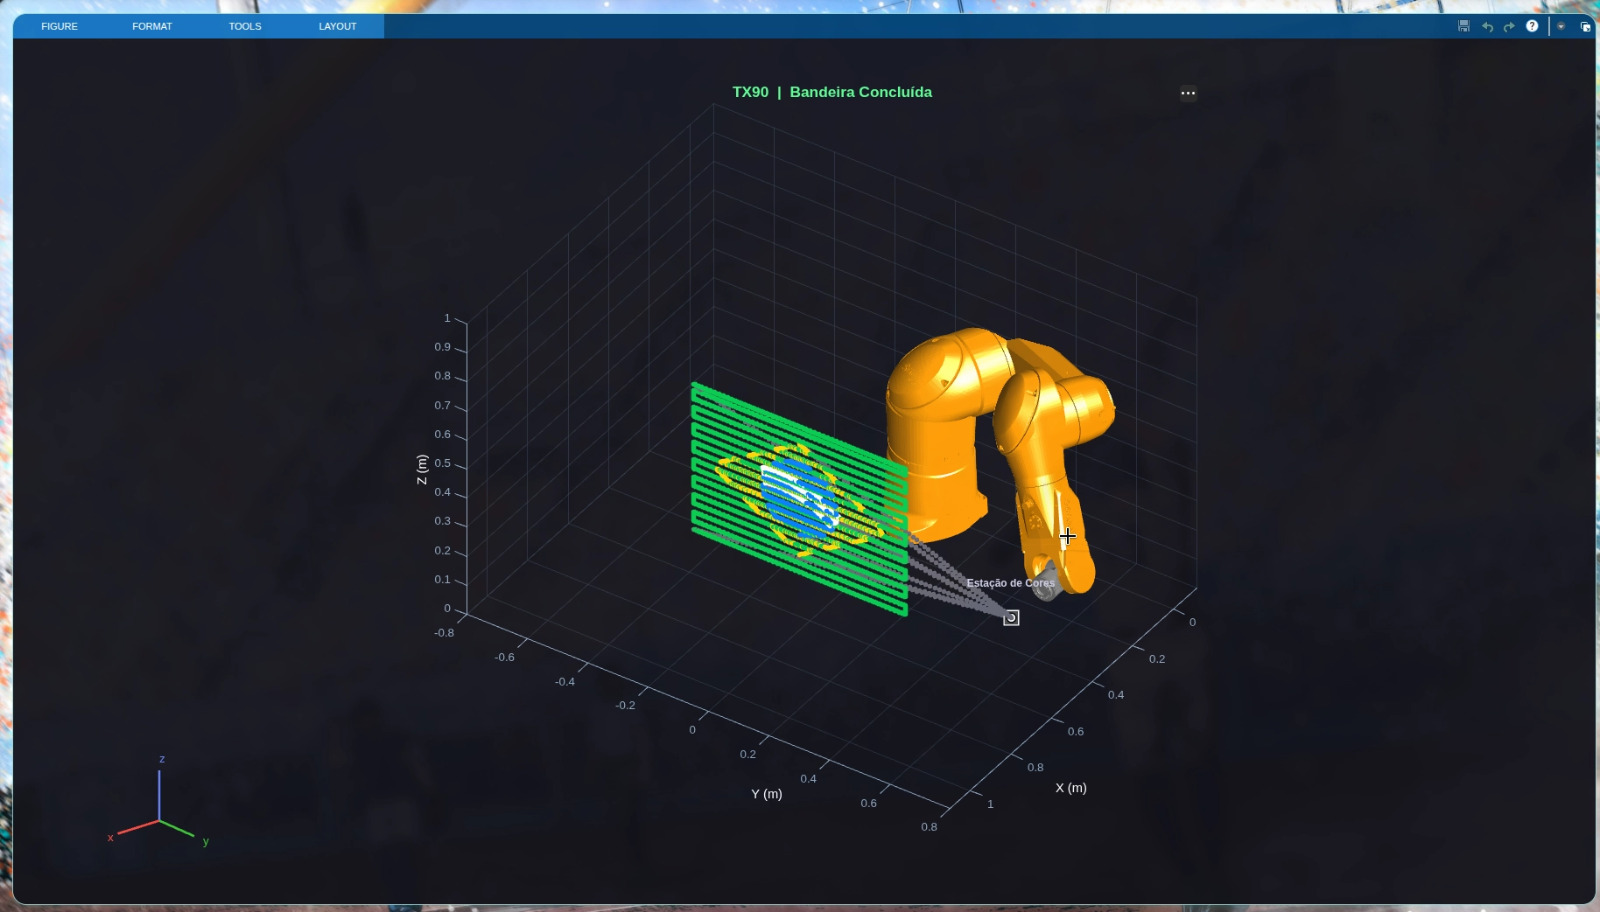
\includegraphics[width=0.78\linewidth]{Imagens/bandeira_serpentina.png}}\\[4pt]
    \subfloat[Bandeira preenchida ao final da execução.]{%
        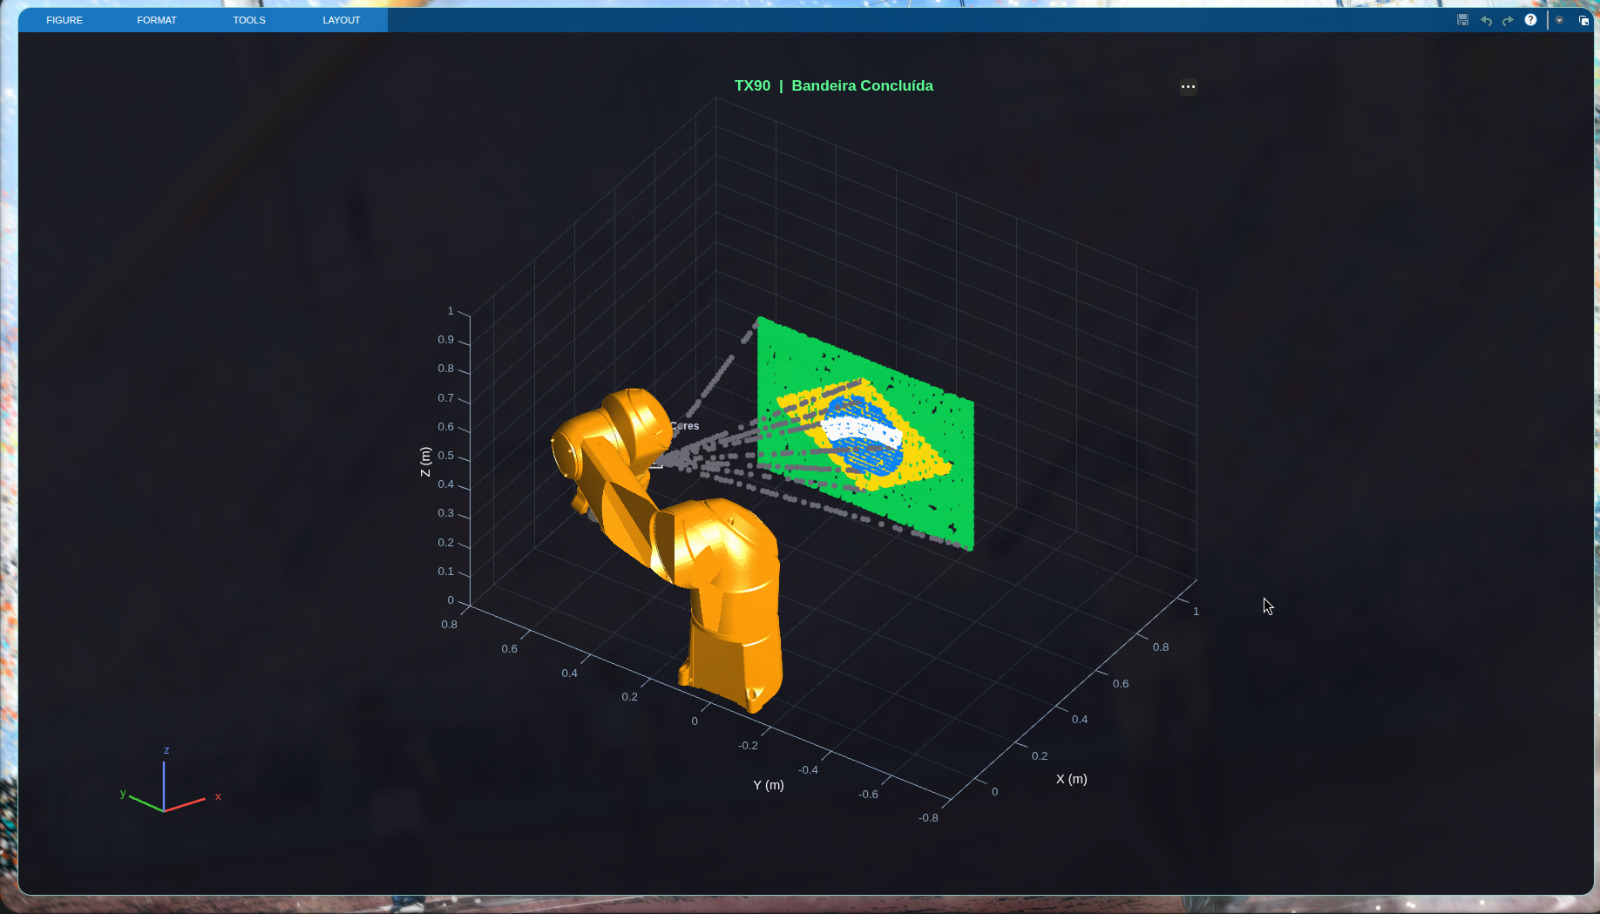
\includegraphics[width=0.78\linewidth]{Imagens/bandeira_preenchida.png}}
    \caption{Preenchimento da bandeira por varredura em serpentina executado pelo TX90.}
    \label{fig:preenchimento}
\end{figure}

Quanto menores forem esses valores, maior será a proximidade entre a trajetória cartesiana desejada e a trajetória realizada pelo manipulador, aumentando a qualidade do nosso controle e permitindo uma movimentação mais equilibrada e fluída.